\section{Coarse-grained simulations}

\begin{figure}[ht]
  \begin{centering}
  \adjustbox{minipage=1.3em,valign=t}{\subcaption{}\label{sfig:testa}}%
  \begin{subfigure}[t]{\dimexpr.4\linewidth-1.3em\relax}
  \centering
  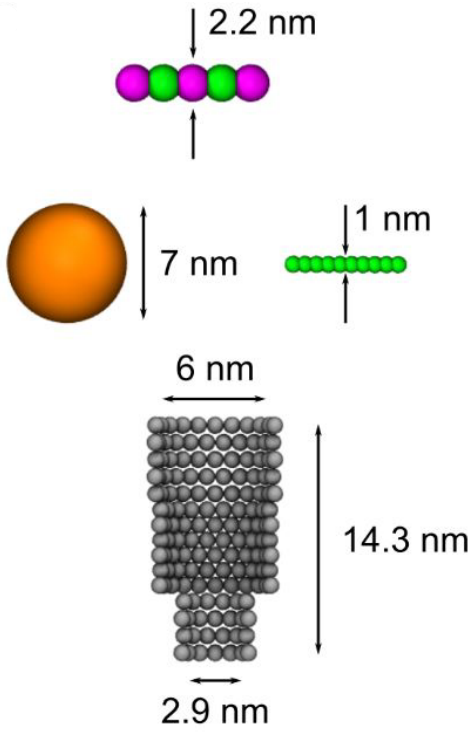
\includegraphics[width=0.9\linewidth,valign=t]{Figures/Stefanos1.png}
  \end{subfigure}%
  \adjustbox{minipage=1.3em,valign=t}{\subcaption{}\label{sfig:testb}}%
  \begin{subfigure}[t]{\dimexpr.5\linewidth-1.3em\relax}
  \centering
  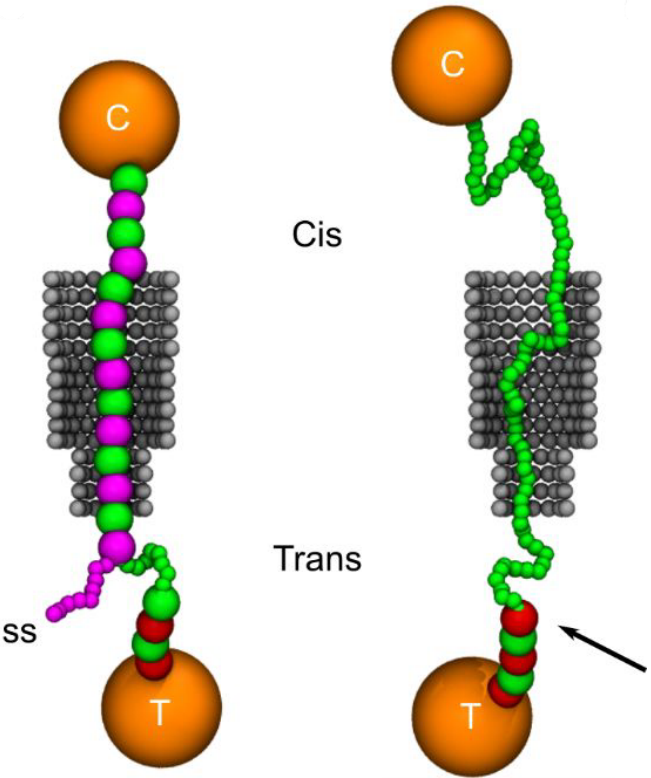
\includegraphics[width=0.9\linewidth,valign=t]{Figures/Stefanos2.png}
  \end{subfigure}
  \caption{This is a figure}
  \label{fig:test}
  \end{centering}
\end{figure}


Undertanding the Entropic interactions + providing a way to look into detail what
happens. Chemist only measure current, we can provide a new window into the world of the
nanopore.

LAMMPS.

Discuss bead spring model DNA + repulsive LJ interactions to simulate excluded volume
interactions.

The bond strength is chosen to be, by transforming the equation for persistence length
kSsDNA = persistenceSsDNA * boltzmann * temperature / lengthNt
kDsDNA = persistenceDsDNA * boltzmann * temperature / lengthBp
$k_{bend} = l_p * k_{bt} * T / \langle a \rangle$
Kuhn segments for ssDNA en dsDNA are different!

Gaussian probably distribution of the beads, i.e. the beads show ideal chain behaviour.
Equipartition theorem.

$k_{bond} = 3 k_b T / \langle a \rangle$

Design nanopore and neutravidin pore. Based on electrostatic calculations + size stopper
is fittud using simulations, requiring blockage to occur.

Langevin integrator is used As is common in simula- tions of coarse-grained models, we
use a higher diffusion coefficient than for physical DNA.

discuss limits of the model. Limited accuracy of the CG model since it does not caputre
the full structure of DNA accurately. For example the double helix structure is note
captured. Another consequence is that the DNA hybridisation can not be simulated using
this model, since both ssDNA nucleotides and dsDNA basepairs are represented by simple
beads. To further analyse and understand the operation cycle of the nanopiston a more
accurate CG model is nodig.

Static clya nanopore made
out of three cylinders. oxDNA strand simulating the DNA connected to the neutravidin
beads represented as spherical beads connected with harmonic springs to the DNA. the
spring constant is determined by using the equipartition theorem. The lipid bi layer in
which the pore is embedded is simulated by a reflective boundary at the lower entrance of
the nanopore interacting only with the neutravidin beads.
